\documentclass{standalone}
\usepackage{tikz}
\usepackage{ctex,siunitx}
\usepackage{tkz-euclide}
\usepackage{amsmath}
\usetikzlibrary{patterns, calc}
\usetikzlibrary {decorations.pathmorphing, decorations.pathreplacing, decorations.shapes,}
\begin{document}
\small
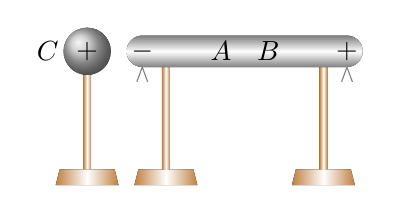
\begin{tikzpicture}[>=latex,scale=1.0]
  % \useasboundingbox(-1,-2)rectangle(8,6);
  \fill[left color=brown,right color=brown, middle color=white](-0.05,0)rectangle(0.05,-1.5);
  \fill[ball color=lightgray](0,0)circle(0.3)node{$+$};
  \node at(-0.5,0){$C$};
  \fill[left color=brown,right color=brown, middle color=white](-0.4,-1.7)--(-0.35,-1.5)--(0.35,-1.5)--(0.4,-1.7)--cycle;
  \begin{scope}[xshift=1cm]
    \fill[left color=brown,right color=brown, middle color=white](-0.4,-1.7)--(-0.35,-1.5)--(0.35,-1.5)--(0.4,-1.7)--cycle;
    \fill[left color=brown,right color=brown, middle color=white](-0.05,0)rectangle(0.05,-1.5);
    \fill[top color=gray,bottom color=gray, middle color=white](1,0.2)--(-0.3,0.2)arc(90:270:0.2)--(1,-0.2)--cycle;
    \draw[gray](-0.3,-0.2)--++(250:0.2)(-0.3,-0.2)--++(290:0.2);
    \node at (-0.3,0){$-$};
    \node at (0.7,0){$A$};
  \end{scope}
  \begin{scope}[xshift=3cm]
    \fill[left color=brown,right color=brown, middle color=white](-0.4,-1.7)--(-0.35,-1.5)--(0.35,-1.5)--(0.4,-1.7)--cycle;
    \fill[left color=brown,right color=brown, middle color=white](-0.05,0)rectangle(0.05,-1.5);
    \fill[top color=gray,bottom color=gray, middle color=white](-1,0.2)--(0.3,0.2)arc(90:-90:0.2)--(-1,-0.2)--cycle;
    \draw[gray](0.3,-0.2)--++(250:0.2)(0.3,-0.2)--++(290:0.2);
    \node at (0.3,0){$+$};
    \node at (-0.7,0){$B$};
  \end{scope}
\end{tikzpicture}
\end{document}